\documentclass[a4paper]{jpconf}
\usepackage{graphicx}
\usepackage{url}
\usepackage{hepparticles}
\usepackage[nomargin,inline,marginclue,draft]{fixme}

\begin{document}
\title{A novel method for event reconstruction in Liquid Argon Time Projection Chamber}

\author{M Diwan, M Potekhin, B Viren, X Qian and C Zhang}

\address{Brookhaven National Laboratory, Upton, NY11973, USA}

\ead{xqian@bnl.gov}


\begin{abstract}
Future experiments such as the Deep Underground Neutrino Experiment (DUNE) will use very large
Liquid Argon Projection Chambers (LArTPC) containing tens of kilotons of cryogenic medium. To be able to utilize
sensitive volume  of that size, current design employs arrays of wire electrodes
grouped in readout planes, arranged with a stereo angle. This leads to certain challenges for object reconstruction
due to ambiguities inherent in such a scheme. We present a novel reconstruction method (named ``Wirecell')
inspired by principles used in tomography, which brings the LArTPC technology closer to its full potential.
\end{abstract}

\section{Introduction}

The new method of event reconstruction in Liquid Argon Time Projection Chamber (LArTPC) presented here
is motivated by the stringent requirements of the DUNE experiment~\cite{cdrVol1}. The DUNE primary science
program~\cite{cdrVol2} includes precision measurements of the parameters that govern neutrino oscillations,
search for proton decay, and detection and measurement of the \HepParticle{\nu}{e}{} flux from a core-collapse supernova in our galaxy.
One of the central components of DUNE is a massive Far Detector (40kt fiducial volume) based on Liquid Argon Time Projection Chamber (LArTPC)
located deep underground at a distance of 1,300\,km from the neutrino source~\cite{cdrVol4}.
This device  has the potential to reconstruct tracks and showers with  high level of detail and  efficiency,
as well as to provide a precise measurement of ionization charge necessary for good particle identification based on ionization energy loss ($dE/dx$).
The single-phase LArTPC design which is our focus here is an ionization chamber with multi-wire readout and no amplification in the medium,
which is cryogenic liquid Argon.  For a very large detector like DUNE using pads for readout is not practical, and the liquid argon volume is
instrumented with planar arrays of wire electrodes.

\section{Operation of the LArTPC with wire readout}
\subsection{Principle of Operation}
The LArTPC volume is instrumented with sensor wires which in case of DUNE are spaced at a $\sim$4.5\,mm pitch, and configured 
as planar arrays forming induction and collection planes. The planes are aggregated into structural units called Anode Plane Assemblies,
or APAs. Each side of the APA contains two induction planes and one collection plane, in a stereo angle configuration illustrated in
Fig.\ref{fig:wireplanes1} which is a schematic view of the APA along the drift direction (i.e. line of sight is perpendicular to the APA).
\begin{figure}[h!]
	\centering
	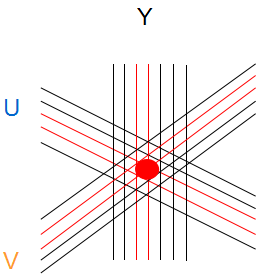
\includegraphics[width=0.45\textwidth]{uvy_3.png}
	\caption{Collection and Induction Wire Planes as viewed along the drift direction}
	\label{fig:wireplanes1}
\end{figure}

\noindent
In this diagram, arrays of wires labeled ``U'' and ``V'' represent the two induction planes, while ``Y'' wires constitute the
collection plane, i.e. the electrodes where ionization electrons are collected after completing their drift in the liquid argon medium.
Every induction and collection wire is read out as an individual channel, with waveforms recorded at $\sim$2\,MHz digitization frequency.
There are also planar Cathode Plane Assemblies which are necessary to create a near-uniform electrostatic field in
the chamber, however they are not instrumented. The dot in the center of the diagram represents a localized ionization charge
which creates signals on wires in all three planes (U,V,Y).

The LArTPC principle of operation is schematically illustrated in Fig.\ref{fig:lartpc-principle}.
In this diagram, ionization electrons are
produced in the medium by a few tracks associated with an event. They start drifting to the right, while
positive ions travel towards the cathode on the left hand side. Drifting electrons produce signals on the induction planes ``U''
and ``V'', and  on the collection wire plane ``Y''. The ionization pattern can then be reconstructed
 in the plane perpendicular to the drift direction by analyzing signals on (U,V,Y). 
\begin{figure}[h!]
	\centering
	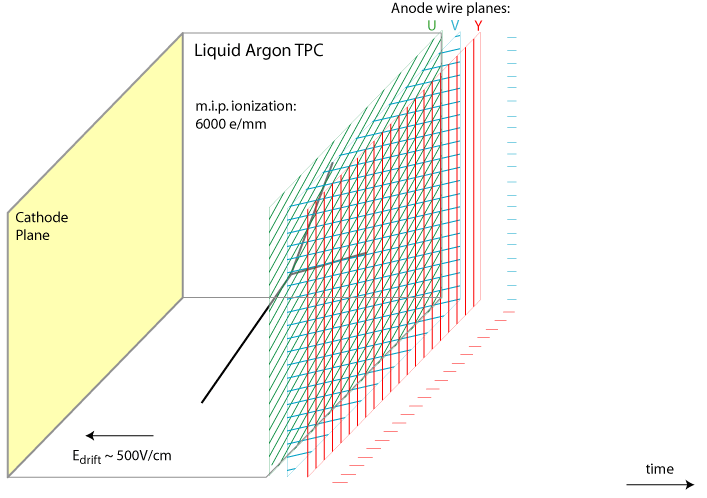
\includegraphics[width=0.7\textwidth]{signal-0.png}
	\caption{The LArTPC Principle of Operation}
	\label{fig:lartpc-principle}
\end{figure}
Reconstruction along the axis of the drift direction
can be done using the information contained in the time evolution of the signals on the (U,V,Y) wire planes, since each time bin corresponding to the
ADC digitization cycle can be mapped to the coordinate in that direction, through the known (calibrated) value of drift velocity.

In general, signals on individual wires produce complex waveforms, and are subject to electronics noise, shaping parameters in the
amplifier chain and other factors. Evaluating the charge in a particular time bin involves complex signal processing, and
is beyond the scope of this paper.

\subsection{The Challenge}
\label{ambiguity}
It is not difficult to see that while the wire readout design makes construction of very large LArTPCs possible by keeping the channel count
within practical limits,
it does so at the cost of information loss, since now instead of pads or pixels one has to reconstruct the position of the
particle ``hits'' in 2D using three projections. If the number of sensor wires that
registered a signal is $\sim$N, the number of potential hit locations scales as $\sim$N$^2$, which naturally leads to ambiguities.



\section{The ``Wirecell'' method}
\subsection{Reconstruction in LArTPC}
Event reconstruction in LArTPCs with wire readout is primarily geared towards neutrino interactions
with multiple final state particles emerging from  a single vertex. 
Reconstruction methods which existed prior to introduction of the method described in this paper were inspired by tracking
algorithms utilized in High Energy Physics, and indeed reused existing software libraries
in some cases. A typical approach starts with identifying track candidates in each of the three projections which were described
above. This is done by identifying groups of wires in each projection which had ``hits'' is adjacent time bins, effectively relying
on the continuity of the object being reconstructed at this stage in the reconstruction process. Hypotheses are applied regarding
whether the object corresponds to a track or to a shower. Then, an attempt is made to match individual 2D (time-coordinate)
projections in 3D\,\cite{icarus}. As mentioned in \ref{ambiguity}, there are ambiguities in this process which result in
reconstruction artifacts such as ghost tracks etc.


\subsection{Parallels to Tomography}
The method of collecting signals from LArTPC has  parallels with Computerized Axial Tomography
(CAT) applications. Each time slice in LArTPC is
digitized separately and effectively represents a separate unit of data. This can be compared to one of the original (and simplest) methods of CAT
called Multiplanar Reconstruction -- MPR -- in which the volume under study is treated as a stack of 2D slices. Revisiting
Fig.\ref{fig:wireplanes1} one can see that the same charge pattern in an individual 2D slice is sampled in three different projections.
Each wire is  measuring a line integral of the ionization charge located in its vicinity. This has significant similarity
to absorption tomography where attenuation of radiation intensity also corresponds to a line integral along
the direction of the beam. Clearly, the number of projections is extremely limited (to three) which makes application of mainstream
CAT reconstruction techniques such as Radon transform ~\cite{radon1}
not practical. It must be noted however that sparse and limited-angle tomography
does have its applications and domain-specific mathematical methods have been developed to deal with such extremely ill-posed problems.

CAT applications typically feature voxelization of the object under study due to natural granularity of the apparatus and also to make numerical
calculations feasible. In multiplanar reconstruction, this effectively leads to treating each individual 2D slice as a set of pixels, defined according
to the type of measurement. Application of this technique (introduction of cells) is the foundation of the Wirecell method
for LArTPC
described here\,\cite{wirecell}.


\subsection{The ``Wirecell'' algorithm}
In Wirecell, a tessellation algorithm is used to describe each 2D time-slice (defined by a single time bin of the ADCs processing the signals
from wire planes) as a set of polygon pixels. Each wire is associated with a subset of pixels.
The wire signals now have to processed in the next two steps: 
\begin{itemize}
\item Solving the inverse problem in each 2D slice, i.e. performing 2D imaging (reconstructing pixel values) using the three projections of the
charge distribution in the time slice.
\item Combining the 2D slices to obtain a 3D model of the ionization pattern in the Liquid Argon Volume, which can then be used to extract
physics information about the event.
\end{itemize}

\noindent
The inverse problem of determining pixel charge values based on limited number of projections (three sets of wires) is  ill-posed.
Therefore, the following algorithm is applied: groups of adjacent candidate cells with signal above a 
threshold are identified. They are grouped into ``merged cells'' (i.e. the charge values are combined to effectively form a larger pixel).
Note that many of these cells will be effectively ghosts due ambiguities as described above  (see~\ref{ambiguity}).
Wires mapped to these merged cells are also merged. This results in reduction of the number of degrees of freedom. Signals on merged wires
are observed experimentally, while the values of the charge in merged cells are not due to ambiguities. The relationship
between the two can be represented as $W_m=G$\,$C_m$, where $W_m$ is the vector of values attributed to charges on merged wires, $G$ is
the geometry matrix mapping wires to cells, and the $C_m$ is the vector of values for merged cells, for which a solution must be found. In vast majority
of cases this cannot be solved by matrix inversion. Instead, the Wirecell method employs the Markov Chain Monte Carlo (MCMC) approach, which aims
to minimize the following value:
$$\chi^2=(W_m-GC_m)^TV^{-1}(W_m-GC_m)$$
$V$ stands for the covariance matrix for signals on merged wires.
Each step in the MCMC process involves removing a random cell and recalculating $G$ to evaluate the metric as described above. If the $\chi^2$ value
improves, such cell is permanently eliminated under the hypothesis that it was a ``ghost cell''. Once a sufficient number of cells have been eliminated,
matrix inversion becomes possible which completes the solution. A reconstructed 2D image is formed, and a stack of these images forms the 3D
picture of the physics event in LArTPC. It is important to note that in this method, no physics assumptions are made either about the type of particle
or the number of tracks in the event before the event is assembled in 3D.  Nevertheless, statistical fluctuations may in some cases result in non-convergence
or mis-reconstruction.  

Optimization technique as described above can be modified to take advantage of apriori information about the object, which is another common
approach in the field of tomography. For example the hypothesis of object continuity in 3D can be included in the solution by adding a penalty
value to $\chi^2$ in cases there there are no active cells in neighboring 2D slices, adjacent to the one being considered for elimination during the MCMC step.

The Wirecell algorithm contains a number of elements which are computationally intensive, e.g. each step in the Markov Chain involves recalculating
matrices and other operations. For that reason, work is currently under way to adapt Wirecell for use on modern parallel computing platforms,
including GPUs.

\subsection{Status and future directions}
The Wirecell method has been applied to reconstruction of a variety of event classes using Monte Carlo data. In the first round of analysis,
efficiency of track reconstruction in this method is at or above the levels stipulated by the requirements of the DUNE experiment.
It is currently being adapted for
event reconstruction in the $\mu$BooNE experiment~\cite{uboone}, and results are expected to become available soon.
\begin{figure}[h!]
	\centering
	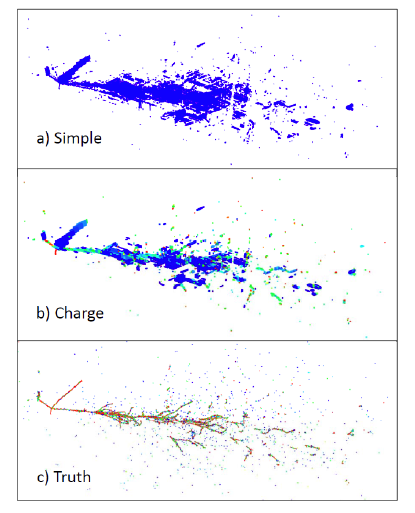
\includegraphics[width=0.5\textwidth]{wirecell_vs_mc.png}
	\caption{Comparison of hit-based reconstruction (``simple''), Wirecell (``charge'') and MC Truth (``truth'')}
	\label{fig:wirecell_vs_mc}
\end{figure}



\section{Summary}
A novel reconstruction method has been developed which applies tomography principles to
neutrino event reconstruction in Liquid Argon Time Projection Chambers with
wire readout. Markov Chain Monte Carlo technique is used for the inverse problem solution in 2D, with a full 3D image formed as a stack of 2D slices.
First results are promising and indicate that this method can bring the LArTPC technology closer to its full potential for physics research.


\section*{References}
\begin{thebibliography}{9}
\bibitem{cdrVol1} DUNE CDR Vol 1 -- The LBNF and DUNE Projects: \url{http://arxiv.org/abs/1601.05471}
\bibitem{cdrVol2} DUNE CDR Vol 2 -- The Physics Program for DUNE at LBNF: \url{http://arxiv.org/abs/1512.06148}
\bibitem{cdrVol4}  DUNE CDR Vol 4 -- The DUNE Detectors at LBN:F \url{http://arxiv.org/abs/1601.02984}
\bibitem{icarus}  F. Arneodo et al. (The ICARUS-Milano Collaboration) ``Performance Of A Liquid Argon Time Projection Chamber Exposed To The WANF Neutrino Beam'', Phys.Rev.D74:112001,2006
\bibitem{radon1}  William H. Press, `` Discrete Radon transform has an exact, fast inverse and generalizes to operations other than sums along lines'', Proceedings of the National Academy of Sciences of the United States of America, 19249–19254, doi: 10.1073/pnas.0609228103
\bibitem{wirecell} Wirecell: \url{http://www.phy.bnl.gov/wire-cell/}
\bibitem{uboone} $\mu$BooNE experiment: \url{http://www-microboone.fnal.gov}

\end{thebibliography}

\end{document}


